\documentclass [12pt]{article}

\usepackage{tikz}
\usetikzlibrary{positioning}
\usepackage{listings}

\usepackage{xcolor}

\definecolor{codegreen}{rgb}{0,0.6,0}
\definecolor{codegray}{rgb}{0.5,0.5,0.5}
\definecolor{codepurple}{rgb}{0.58,0,0.82}
\definecolor{backcolour}{rgb}{0.95,0.95,0.92}

\lstdefinestyle{verilog_style}{
    backgroundcolor=\color{backcolour},   
    commentstyle=\color{codegreen},
    keywordstyle=\color{magenta},
    numberstyle=\tiny\color{codegray},
    basicstyle=\ttfamily\footnotesize,
    breakatwhitespace=false,         
    breaklines=true,                 
    captionpos=b,                    
    keepspaces=true,                 
    numbers=left,                    
    numbersep=5pt,                  
    showspaces=false,                
    showstringspaces=false,
    showtabs=false,                  
    tabsize=2
}

\lstset{style=verilog_style}

\title {\textbf{RAM - ROM PRESENTATION}}

\author{Pham Duc Anh Khoa - 2053140 \\
				Nguyen Thi Ngoc Nhi - 2052632\\
				Ngo Chan Phong - 2053321 \\
				Le Hoang Minh - 2052595 \\
				Tran Hoang Minh Quan - 2053380 \\
				Phan Tien Vinh - 2052323\\
				Nguyen Tien Trung - 2052353}
\date{13 - 05 - 2021}

\begin {document}
	\pagenumbering {gobble}
	\maketitle 
	\newpage
	\pagenumbering {arabic}

	\section {ROM}
		\subsection {Definition}
				\begin{itemize}
					\item \textbf{ROM}: stand for \textbf{Read-only Memory}.
					\item Primary memory unit of computer system along with RAM.
					\item Remain with the unit even when the system is powered off.
					\end{itemize}
		\subsection {Structure}
			\begin {itemize}
				\item \textbf{Block Structure}: Below is the block diagram of the Struture\\~\\
				
				% ------- ADDING DIAGRAM ------- %
				
				

\tikzset{every picture/.style={line width=0.75pt}} %set default line width to 0.75pt        

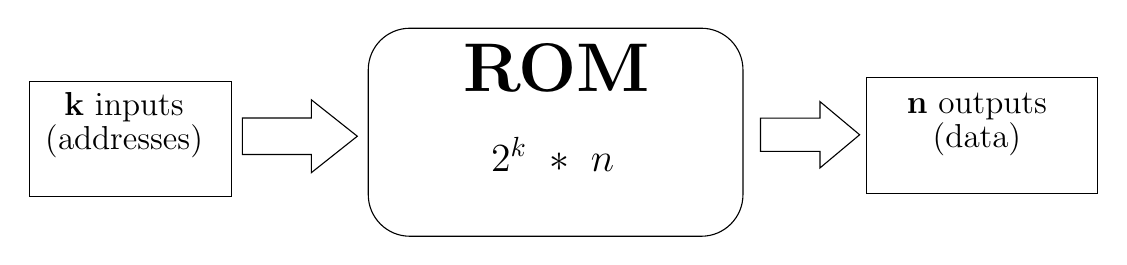
\begin{tikzpicture}[x=0.75pt,y=0.75pt,yscale=-1,xscale=1]
%uncomment if require: \path (0,299); %set diagram left start at 0, and has height of 299

%Rounded Rect [id:dp0964091744319382] 
\draw   (170.27,115.43) .. controls (170.27,104.36) and (179.24,95.38) .. (190.31,95.38) -- (330.76,95.38) .. controls (341.83,95.38) and (350.8,104.36) .. (350.8,115.43) -- (350.8,175.56) .. controls (350.8,186.63) and (341.83,195.6) .. (330.76,195.6) -- (190.31,195.6) .. controls (179.24,195.6) and (170.27,186.63) .. (170.27,175.56) -- cycle ;
%Shape: Rectangle [id:dp3814793707029971] 
\draw   (7,121.07) -- (104.42,121.07) -- (104.42,176.57) -- (7,176.57) -- cycle ;
%Shape: Rectangle [id:dp6349239006386276] 
\draw   (410.37,119.32) -- (521.8,119.32) -- (521.8,174.81) -- (410.37,174.81) -- cycle ;
%Right Arrow [id:dp4359165413489341] 
\draw   (109.63,138.63) -- (142.84,138.63) -- (142.84,129.85) -- (164.99,147.41) -- (142.84,164.98) -- (142.84,156.2) -- (109.63,156.2) -- cycle ;
%Right Arrow [id:dp48219685373969967] 
\draw   (359.23,138.72) -- (387.9,138.72) -- (387.9,130.73) -- (407.01,146.71) -- (387.9,162.69) -- (387.9,154.7) -- (359.23,154.7) -- cycle ;

% Text Node
\draw (214.71,101.72) node [anchor=north west][inner sep=0.75pt]   [align=left] {\textbf{{\Huge ROM}}};
% Text Node
\draw (228.22,146.79) node [anchor=north west][inner sep=0.75pt]  [font=\Large]  {$2^{k} \ *\ n$};
% Text Node
\draw (6.44,125.29) node [anchor=north west][inner sep=0.75pt]   [align=left] {\begin{minipage}[lt]{67.35pt}\setlength\topsep{0pt}
\begin{center}
{\large \textbf{k} inputs}\\{\large (addresses)}
\end{center}

\end{minipage}};
% Text Node
\draw (417.33,125.54) node [anchor=north west][inner sep=0.75pt]   [align=left] {\begin{minipage}[lt]{67.35pt}\setlength\topsep{0pt}
\begin{center}
{\large \textbf{n} outputs}\\{\large (data)}
\end{center}

\end{minipage}};


\end{tikzpicture}


				% ----- END DIAGRAM ------
				
					\item It consist of \textbf{k} input lines and \textbf{n} output lines. 
					
					\item \textbf{k} inputs are in binary form and is used to determine the addresses we want to access inside \textbf{ROM}.
					
					\item Since \textbf{k} inputs is in binary form, we can calculate the total addresses can be referred by the formula: $2^k$.
					
					\item \textbf{n} is the number of bit information that contain in each address line $\Rightarrow$ the size of a \textbf{ROM} can be calculated by the formula: $2^k * n$.
					
					\item \textbf{Internal structure: }\\~\\
					\centerline{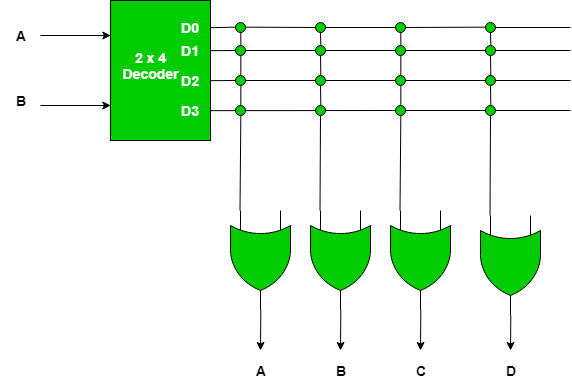
\includegraphics[scale = 0.5]{rom_internal.png}}\\~\\
					
					\item Consists of two components: \textbf{Decoder} and \textbf{Or gates}.
					
					\end {itemize}


		\subsection {How it works ?}
			\begin {itemize}
				\item Let's have a look again at the internal structure: \\~\\
				\centerline{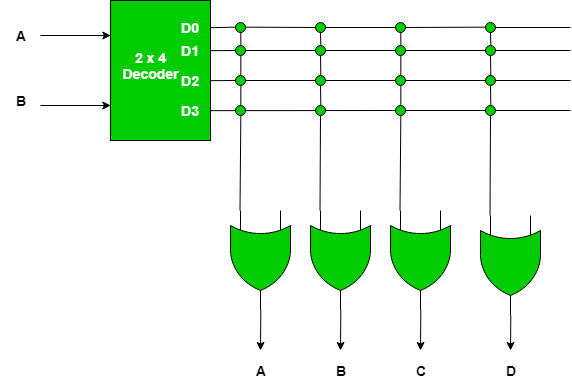
\includegraphics[scale = 0.5]{rom_internal.png}} \\~\\
				
				\item The decoder will decode data from binary form to more known for like decimal.
				
				\item In ROM, the input to a decoder will be in binary form and the output will represent its decimal equivalent .
				
				\item All the OR gates present in the ROM will have outputs of the decoder as their input .
				
				\item All the intersections as shown in the internal structure diagram above can be programmed to meet our demand.
			\end {itemize}


		\subsection{Classification}
			\begin {itemize}
				\item \textbf{PROM}: \\
					- Stands for Programmable ROM.\\
					- Appear as a blank memory unit after manufacturing.\\
					- Can only be programed once, the data will be eternal.\\
					- Suitable for storing eternal data like sound in electronic devices or sound driver in organs...\\
					
				\item \textbf{EPROM}:\\
				- Stands for Erasable Programmable ROM.\\
				- An erasable version of PROM.\\
				- Erasing method:  shortwave radiation under ultra violet light for the length of time.\\
				- Used to be used in old microcontrollers.\\
				
				 \item \textbf{EEPROM}:\\
				- Stands for Electronic Erasable Programmable ROM.\\
				- A version of EPROM that the data inside can be erased by electronic, 1 byte at a time.\\
				- Erasing method:  electrical signal, under ultraviolet light.\\
				- Mostly used for storing old computer BIOS.\\
				
				 \item \textbf{Flash ROM}:\\
				- A better version of EEPROM, 512 bytes of data can be written or erased at a time.\\
				- Much faster than EEPROM.\\
				- Mostly used for storing modern computer BIOS.\\
					
			\end {itemize}
			

		\subsection{Programming the ROM}
		\begin {itemize}
			\item To begin, we have to define what is the value at each address in the ROM. In this example, th following truth table will be use \\
			% TRUTH TABLE
			\begin{table}[!h]
				\centering
				\begin{tabular}{|c|c|}
				\hline
				\textbf{Address} & \textbf{Value} \\ \hline
				00               & 0010           \\ \hline
				01               & 0011           \\ \hline
				10               & 0100           \\ \hline
				11               & 0101           \\ \hline
				\end{tabular}
			\end{table} 
			% END TRUTH TABLE
			
			\item Here is the code for the following definition:\\
			
			\lstinputlisting[language=Verilog]{rom_example.v}
		\end {itemize}
		
		
		\section {RAM}
		
			\subsection{Definition}
			\begin {itemize}
				\item \textbf{RAM} - short for “random access memory”, \textbf{RAM} is used to read and write into memory. 
				
				\item \textbf{RAM} stores files and data of programs that are currently being executed by CPU.
				
				\item \textbf{RAM} is a volatile memory as data loses when power is turned off.
				
				\item The more \textbf{RAM} you have, the better your computer will perform.
			\end{itemize} 
			
			\subsection{Structure}
				\begin {itemize}
					\item \textbf{Block structure} - below is the block diagram of \textbf{RAM}:
					
					% ADD DIAGRAM
						

\tikzset{every picture/.style={line width=0.75pt}} %set default line width to 0.75pt        

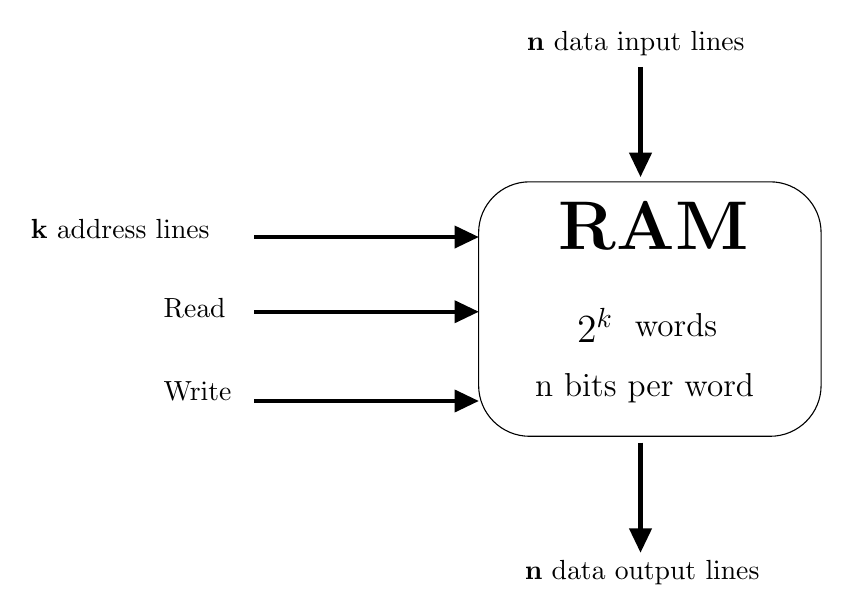
\begin{tikzpicture}[x=0.75pt,y=0.75pt,yscale=-1,xscale=1]
%uncomment if require: \path (0,300); %set diagram left start at 0, and has height of 300

%Rounded Rect [id:dp5971964868164206] 
\draw   (251,112.52) .. controls (251,98.98) and (261.98,88) .. (275.52,88) -- (391.48,88) .. controls (405.02,88) and (416,98.98) .. (416,112.52) -- (416,186.08) .. controls (416,199.62) and (405.02,210.6) .. (391.48,210.6) -- (275.52,210.6) .. controls (261.98,210.6) and (251,199.62) .. (251,186.08) -- cycle ;
%Straight Lines [id:da9905792719063355] 
\draw [line width=1.5]    (329,32.6) -- (329,81.6) ;
\draw [shift={(329,85.6)}, rotate = 270] [fill={rgb, 255:red, 0; green, 0; blue, 0 }  ][line width=0.08]  [draw opacity=0] (11.61,-5.58) -- (0,0) -- (11.61,5.58) -- cycle    ;
%Straight Lines [id:da9049928349701912] 
\draw [line width=1.5]    (329,213.6) -- (329,262.6) ;
\draw [shift={(329,266.6)}, rotate = 270] [fill={rgb, 255:red, 0; green, 0; blue, 0 }  ][line width=0.08]  [draw opacity=0] (11.61,-5.58) -- (0,0) -- (11.61,5.58) -- cycle    ;
%Straight Lines [id:da5383676500951724] 
\draw [line width=1.5]    (143,114.6) -- (247,114.6) ;
\draw [shift={(251,114.6)}, rotate = 180] [fill={rgb, 255:red, 0; green, 0; blue, 0 }  ][line width=0.08]  [draw opacity=0] (11.61,-5.58) -- (0,0) -- (11.61,5.58) -- cycle    ;
%Straight Lines [id:da5149347484239479] 
\draw [line width=1.5]    (143,150.6) -- (247,150.6) ;
\draw [shift={(251,150.6)}, rotate = 180] [fill={rgb, 255:red, 0; green, 0; blue, 0 }  ][line width=0.08]  [draw opacity=0] (11.61,-5.58) -- (0,0) -- (11.61,5.58) -- cycle    ;
%Straight Lines [id:da5750709401561154] 
\draw [line width=1.5]    (143,193.6) -- (247,193.6) ;
\draw [shift={(251,193.6)}, rotate = 180] [fill={rgb, 255:red, 0; green, 0; blue, 0 }  ][line width=0.08]  [draw opacity=0] (11.61,-5.58) -- (0,0) -- (11.61,5.58) -- cycle    ;

% Text Node
\draw (288.45,96.37) node [anchor=north west][inner sep=0.75pt]   [align=left] {\textbf{{\Huge RAM}}};
% Text Node
\draw (297.22,147.79) node [anchor=north west][inner sep=0.75pt]  [font=\Large]  {$2^{k}$};
% Text Node
\draw (325,150) node [anchor=north west][inner sep=0.75pt]   [align=left] {{\large words}};
% Text Node
\draw (277,179) node [anchor=north west][inner sep=0.75pt]   [align=left] {{\large n bits per word}};
% Text Node
\draw (273,14) node [anchor=north west][inner sep=0.75pt]   [align=left] {\textbf{n} data input lines};
% Text Node
\draw (272,269) node [anchor=north west][inner sep=0.75pt]   [align=left] {\textbf{n} data output lines};
% Text Node
\draw (34,105) node [anchor=north west][inner sep=0.75pt]   [align=left] {\textbf{k} address lines};
% Text Node
\draw (98,143) node [anchor=north west][inner sep=0.75pt]   [align=left] {Read};
% Text Node
\draw (98,183) node [anchor=north west][inner sep=0.75pt]   [align=left] {Write};

\end{tikzpicture}
					% END DIAGRAM
					
					\item The n data input lines provide the information to be stored in memory.
					\item The n data output lines supply the information coming out of the chosen word among the $2^k$ available inside the memory. 
					\item The two control inputs specify the direction of transfer desired.
					
					\item Internal structure of RAM: \\
					\centerline{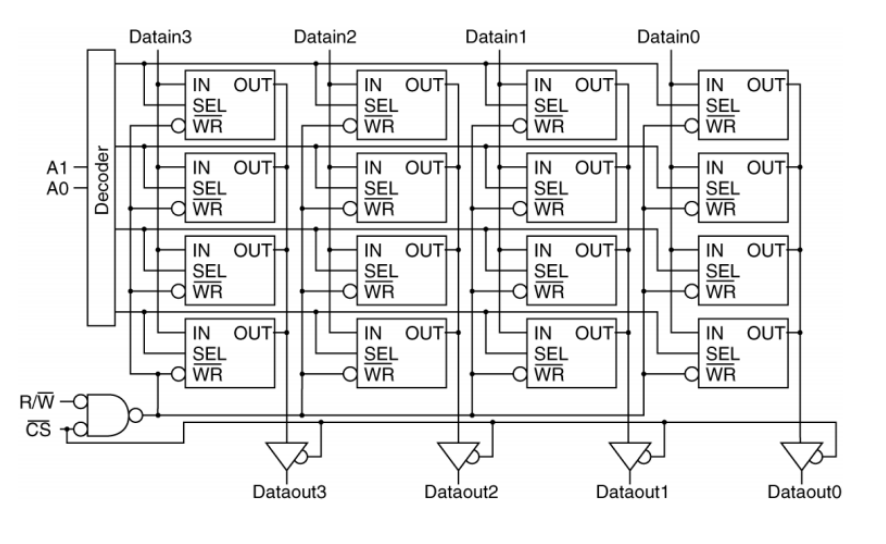
\includegraphics[scale = 0.5]{ram_internal.png}}
				\end{itemize}
				
		\subsection{How it works ?}
			\textbf{RAM} has 2 operations:
				\begin{itemize}
					\item Read function: \\
					- Apply the binary address of the desired word into the address lines.\\
					- Apply the data bits that must be stored in memory into the data input lines.\\
					- Activate the write input.
					
					\item Then the memory unit will then take the bits presently available in the input data lines and store them in the specified by the address lines. 
					
					\item Write function: Specifies a transfer-in operation and the read function specifies a transfer-out operation, in detail: \\
					- Apply the binary address of the desired word into the address lines.\\
					- Activate the read input.
					
					\item Then the memory unit will then take the bits from the word that has been selected by the address and apply them into the output data lines. The content of the selected word does not change after reading.
					
					\end{itemize}

		\subsection {Classification}
		\textbf{RAM} is further classified into two types: \textbf{SRAM} (Static Random Access Memory) and \textbf{DRAM} (Dynamic Random Access Memory)

			\begin {itemize}
				\item \textbf{Static RAM, or (SRAM)}: \\
				- Data is stored in transistors and requires a constant power flow.\\
				- Because of the continuous power, SRAM doesn’t need to be refreshed to remember the data being stored.
				
				\item \textbf{Dynamic RAM, or (DRAM)}:\\
				- Data is stored by using a pair of transistor and capacitor which constitute a DRAM memory cell.\\
				- Capacitors that store data in DRAM gradually discharge energy, no energy means the data has been lost. \\
			\end {itemize}

			Summary of classification:\\
			
			\begin{table}[!h]
			\centering
\begin{tabular}{|l|l|}
\hline
\multicolumn{1}{|c|}{\textbf{DRAM}}                                                                        & \multicolumn{1}{c|}{\textbf{SRAM}}                                                          \\ \hline
\begin{tabular}[c]{@{}l@{}}Constructed of tiny capacitors \\ that leak electricity.\end{tabular}           & \begin{tabular}[c]{@{}l@{}}Constructed of circuits \\ similar to D flip-flops.\end{tabular} \\ \hline
\begin{tabular}[c]{@{}l@{}}Requires a recharge every few \\ milliseconds to maintain its data\end{tabular} & \begin{tabular}[c]{@{}l@{}}Hold its contents as long \\ as power is available\end{tabular}  \\ \hline
Inexpensive.                                                                                               & Expensive.                                                                                  \\ \hline
Slower than SRAM.                                                                                          & Faster than DRAM.                                                                           \\ \hline
Can store many bits per chip.                                                                              & Can not store many bits per chip.                                                           \\ \hline
Uses less power.                                                                                           & Uses more power.                                                                            \\ \hline
Generates less heat.                                                                                       & Generates more heat.                                                                        \\ \hline
Used for main memory.                                                                                      & Used for cache.                                                                             \\ \hline
\end{tabular}
\end{table}

			
\end {document}